\documentclass[11pt]{article}

% ---------------------------------------------------------------------------
% Packages
% ---------------------------------------------------------------------------
\usepackage[utf8]{inputenc}
\usepackage[T1]{fontenc}
\usepackage[margin=1in]{geometry}
\usepackage{amsmath}
\usepackage{amssymb}
\usepackage{booktabs}
\usepackage{multirow}
\usepackage{array}
\usepackage{tabularx}
\usepackage{graphicx}
\usepackage{subcaption}
\usepackage{xcolor}
\usepackage[numbers,sort&compress]{natbib}
\usepackage[colorlinks=true, linkcolor=blue, citecolor=blue, urlcolor=blue]{hyperref}
\usepackage{cleveref}

% ---------------------------------------------------------------------------
% Convenience macros for the Discussion's RESULT / INTERPRETATION / HYPOTHESIS
% discipline (Deliverable I in the accompanying research package).
% ---------------------------------------------------------------------------
\newcommand{\Result}[1]{\par\smallskip\noindent\textbf{Result.} #1\par}
\newcommand{\Interpretation}[1]{\noindent\textbf{Interpretation.} #1\par}
\newcommand{\Hypothesis}[1]{\noindent\textbf{Hypothesis.} #1\par\smallskip}

\title{Zero-Shot Time-Series Foundation Models for Vegetation Forecasting:\\
A Systematic Evaluation of Chronos-2 for Leaf Area Index Prediction,\\
Its Robustness, and the Limits of Adaptation}

% TODO: author list, affiliations, and correspondence not specified in the
% source request -- fill in before submission. Do not fabricate.
\author{Author Name(s) TODO \\ \small Affiliation TODO}
\date{}

\begin{document}

\maketitle

\begin{abstract}
Leaf Area Index (LAI) is a fundamental variable in land--atmosphere modeling, agricultural
monitoring, and drought assessment, and forecasting it typically requires purpose-built
statistical or deep-learning models trained on years of location-specific data. We ask whether a
general-purpose, pretrained time-series foundation model (TSFM) -- Amazon's Chronos-2 -- can
forecast LAI competitively \emph{without any task-specific training}, and what its zero-shot use
reveals about robustness, generalization, and the value of subsequent adaptation. Using LAI and
meteorological covariates for U.S.\ vegetation pixels spanning grassland, deciduous, and
evergreen-forest regimes, we compare zero-shot Chronos-2 against eight supervised baselines
(Random Forest, SVM, and five recurrent/convolutional deep-learning architectures, including the
domain-specific AELSTM model), evaluate robustness across eleven held-out years (330 fold
results), test spatial generalization across a 3{,}700\,km transfer, and systematically probe
whether task-specific adaptation -- standard and advanced parameter-efficient fine-tuning (7
methods total), and four architecturally distinct vegetation-composition-conditioning mechanisms
-- can improve on the pretrained baseline. Zero-shot Chronos-2 is the best or statistically
tied-best model on the majority of pixels tested (mean rank 1.33 of 10 on a single held-out year;
3.70 of 10, second only to Random Forest, across all LOYO-CV folds) and generalizes across a
3{,}700\,km spatial transfer with no measurable loss. However, no adaptation method -- seven
distinct parameter-efficient fine-tuning variants, or four vegetation-composition-conditioning
architectures -- improves consistently on the pretrained model; a decisive randomized control shows
that a conditioning head trained on genuine vegetation composition performs statistically
indistinguishably from one trained on randomly shuffled, scientifically meaningless assignments
(paired $t$-test $p=0.245$, $n=70$). We interpret this pattern of evidence -- strong, robust
zero-shot transfer alongside adaptation that adds noise rather than signal -- as evidence that
Chronos-2's pretrained representation is already close to this dataset's achievable ceiling, with
direct implications for how general-purpose TSFMs should be deployed in data-limited Earth-system
applications: as strong zero-shot forecasters first, with adaptation reserved for regimes where
genuinely larger or more diverse target-domain data are available.
\end{abstract}

% =============================================================================
\section{Introduction}
\label{sec:intro}
% =============================================================================

\subsection{Vegetation and LAI forecasting}
\label{sec:intro-lai}

Leaf Area Index -- the one-sided area of leaf tissue per unit ground area -- is a primary control
on canopy photosynthesis, evapotranspiration, and land--atmosphere energy exchange, and is a
standard input to crop-yield, drought, and land-surface models. Forecasting LAI ahead of a
growing season, or under alternative climate scenarios, has historically relied on statistical
regression, tree-based ensembles (Random Forest, \cite{lai_forecasting_TODO}), and increasingly
recurrent or attention-augmented deep-learning architectures trained from scratch per location
\cite{ts_forecasting_survey_TODO}. This project builds directly on one such purpose-built
architecture, AELSTM \cite{aelstm_TODO}, evaluated on the same pixels and covariates used here.

\subsection{The rise of time-series foundation models}
\label{sec:intro-tsfm}

Time-series foundation models (TSFMs) -- large sequence models pretrained on broad, cross-domain
time-series corpora and applied zero-shot to new series -- have recently shown strong generic
forecasting performance without domain-specific training \cite{ansari2024chronos,tsfm_review_TODO}.
Chronos-2 \citep[Amazon, 2025;][]{ansari2025chronos2} is distinguished among these by native,
first-class support for \emph{known future covariates}: rather than only extrapolating a
univariate history, it can condition a forecast on covariates whose future values are already
known -- precisely the structure of a vegetation forecast made with actual (observed, or
scenario) future weather.

\subsection{Research gap}
\label{sec:intro-gap}

TSFMs are extensively benchmarked on generic forecasting suites, but rarely evaluated on
Earth-system or vegetation-specific tasks where (a) covariates carry a known, physically
meaningful future trajectory, (b) target-domain training data is often limited to a handful of
locations and years, and (c) the practical question is not ``can this model forecast at all'' but
``does adapting it to this domain help, or does its pretrained representation already suffice.''
This gap motivates using Chronos-2 as a concrete test case for vegetation LAI forecasting
\cite{earth_system_fm_TODO}.

\subsection{Research questions}
\label{sec:rq}

\begin{description}
  \item[RQ1.] How well does pretrained Chronos-2 perform in zero-shot LAI forecasting?
  \item[RQ2.] How does its performance compare with conventional supervised ML and deep-learning
    baselines trained specifically for this task?
  \item[RQ3.] How robust is Chronos-2 across different years, vegetation regimes, and locations?
  \item[RQ4.] Under what conditions does it perform particularly well or poorly?
  \item[RQ5.] Does task-specific parameter adaptation improve Chronos-2 beyond its pretrained
    zero-shot capability?
  \item[RQ6.] What do these experiments imply for applying general-purpose TSFMs to vegetation
    forecasting?
\end{description}

\subsection{Contributions}
\label{sec:contributions}

\begin{enumerate}
  \item We provide a systematic evaluation of Chronos-2 for vegetation LAI forecasting under
    zero-shot application, benchmarked fairly (raw-observation rescoring) against eight supervised
    baselines across three vegetation regimes and 330 leave-one-year-out cross-validation folds.
  \item We characterize Chronos-2's robustness and generalization behavior -- temporal (across 11
    years), spatial (a 3{,}700\,km transfer test), and failure-mode-specific (a controlled leakage
    diagnostic isolating distribution shift from representational limitation).
  \item We conduct the most extensive adaptation study of Chronos-2 for a domain task to date
    within this project -- seven parameter-efficient fine-tuning methods and four
    vegetation-composition conditioning architectures, including a randomized shuffled-assignment
    control -- and show that none consistently improves on the pretrained zero-shot
    representation, identifying the mechanism (generic capacity-driven noise, not method-specific
    failure) rather than merely reporting the negative result.
\end{enumerate}

% =============================================================================
\section{Related Work}
\label{sec:related}
% =============================================================================

\subsection{Vegetation and LAI forecasting}
\label{sec:related-lai}
\cite{lai_forecasting_TODO} -- statistical/remote-sensing-based LAI estimation and forecasting
literature; AELSTM \cite{aelstm_TODO} as the direct architectural precedent for this project's
baselines; \cite{lai_lstm_2024} as a directly comparable LAI--climate deep-learning precedent
(continental-scale, attention-enhanced LSTM), used in this project's own PFT-conditioning
literature review to sanity-check task framing.

\subsection{Time-series forecasting}
\label{sec:related-ts}
\cite{ts_forecasting_survey_TODO} -- classical statistical methods, tree ensembles, and deep
sequence architectures (LSTM/BiLSTM/GRU/CNN/attention) as used for the baseline suite here.

\subsection{Time-series foundation models}
\label{sec:related-tsfm}
Chronos \citep{ansari2024chronos} and Chronos-2 \citep{ansari2025chronos2} (Ansari et al., Amazon)
are pretrained, general-purpose forecasters; Chronos-2 adds native known-future-covariate support,
the specific capability exercised throughout this paper's task formulation. \cite{tsfm_review_TODO}
for TimesFM, Moirai, and other contemporary TSFMs, for completeness of the related-work landscape
-- not otherwise used in this project's experiments.

\subsection{Foundation models for environmental / Earth-system applications}
\label{sec:related-earth}
\cite{earth_system_fm_TODO} -- this project did not conduct a literature review specific to
Earth-system foundation models; the research gap in \Cref{sec:intro-gap} is stated on the basis of
this project's own search, not a systematic survey, and should be qualified as such in the final
manuscript.

\subsection{Parameter-efficient adaptation}
\label{sec:related-peft}
LoRA \citep{hu2022lora} is the standard parameter-efficient fine-tuning (PEFT) baseline used
throughout. This project's own literature review additionally evaluated DoRA
\citep{liu2024dora}, VeRA \citep{kopiczko2024vera}, IA3 \citep{liu2022ia3}, LN-Tuning (as applied
to Chronos in a small-data healthcare task, \citealp{arxiv2409.11302}), and BitFit
\citep{zaken2022bitfit}, cross-checked directly against the installed Chronos-2 and
\texttt{peft==0.17.1} source for architectural compatibility rather than assumed from the papers
alone. Independent, directly relevant prior evidence -- \citet{arxiv2607.23146}, evaluating
Chronos-2 itself, found zero-shot beats fine-tuning on small datasets, and full fine-tuning
``unreliable\ldots{} consistently degrading performance''; \citet{arxiv2409.11302} found lighter
PEFT methods can match or beat LoRA on Chronos under scarce-data conditions -- both point in the
same direction this paper's own results independently confirm (\Cref{sec:results-adaptation}).

% =============================================================================
\section{Data and Study Design}
\label{sec:data}
% =============================================================================

\begin{figure}[t]
  \centering
  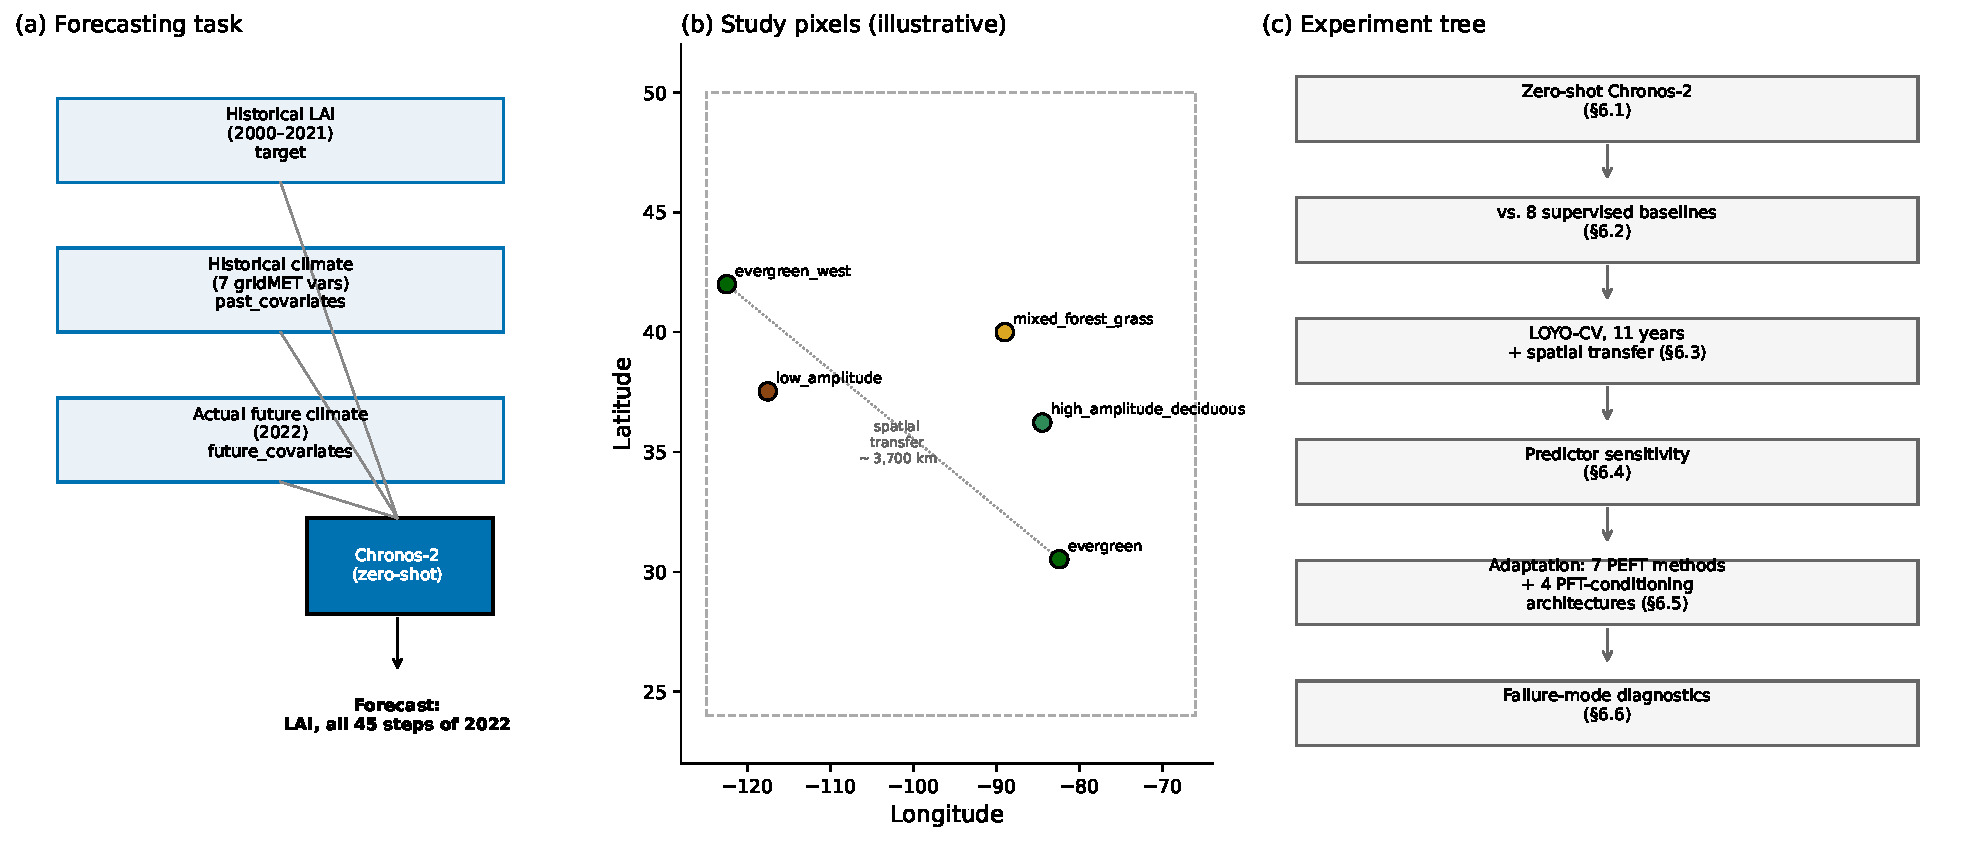
\includegraphics[width=\linewidth]{figures/study_overview.pdf}
  \caption{Overall experimental framework: the forecasting task formulation
  (\Cref{sec:data-formulation}), the study pixels on a CONUS map (\Cref{tab:dataset}), and the
  experiment tree explored in this paper (zero-shot $\rightarrow$ LOYO-CV $\rightarrow$ spatial
  transfer $\rightarrow$ adaptation methods $\rightarrow$ PFT conditioning).}
  \label{fig:study_overview}
\end{figure}

\Cref{fig:study_overview} summarizes the task formulation, study pixels, and experiment tree
described in the remainder of this section.

\subsection{LAI dataset}
\label{sec:data-lai}
HiQ-LAI, 8-day composite, $\sim$1/24\textdegree{} ($\sim$4.6\,km) native grid, continental United
States, 2000--2022.

\subsection{Meteorological covariates}
\label{sec:data-climate}
Seven daily gridMET variables -- maximum/minimum temperature ($\mathit{tmmx}$/$\mathit{tmmn}$),
precipitation ($\mathit{pr}$), downward shortwave radiation ($\mathit{srad}$), vapor pressure
deficit ($\mathit{vpd}$), specific humidity ($\mathit{sph}$), and wind speed ($\mathit{vs}$) --
aligned to each LAI composite's 8-day window by mean, matching the sibling AELSTM project's
established convention exactly.

\subsection{Study locations}
\label{sec:data-pixels}

\Cref{tab:dataset} summarizes the primary study pixels. Three pixels, selected by seasonal-LAI
characteristics alone (never by model performance, per the pixel-selection methodology inherited
from the AELSTM project) anchor the core comparison: \texttt{low\_amplitude} (grassland, smallest
normalized amplitude), \texttt{high\_amplitude\_deciduous} (broadleaf deciduous forest, largest
amplitude among deciduous pixels), and \texttt{evergreen} (needleleaf evergreen forest, flattest
seasonal cycle). Two additional pixels support specific generalization tests: \texttt{evergreen\_%
west} (spatial-transfer target, $\sim$3{,}700\,km from \texttt{evergreen}, same vegetation type)
and \texttt{mixed\_forest\_grass} (PFT-ablation companion pixel, genuinely mixed composition). A
70-pixel pooled set, farthest-point-sampled across a 10-class PFT-composition space with a
geographic minimum-separation constraint, supports the multi-pixel PFT-conditioning experiments.
Three further pixels (\texttt{cropland\_managed}, \texttt{grassland\_shrubland},
\texttt{strong\_interannual\_variability}) were selected by the same methodology but \textbf{have
not been run through Chronos-2} -- an explicit limitation (\Cref{sec:limitations}).

% Table 1: Study pixels, dataset, and forecasting setup
% Source (verified): AELSTM/outputs/pixel_selection/selected_pixels.csv;
%   Chronos2-vegetation-forecasting/Code/common_pipeline.py
\begin{table*}[t]
\centering
\caption{Study pixels, dominant vegetation type, and forecasting setup. LAI target: HiQ-LAI,
8-day composite, $\sim$4.6\,km native grid, continental United States, 2000--2022. Meteorological
covariates: gridMET, 7 daily variables ($\mathit{tmmx}$, $\mathit{tmmn}$, $\mathit{pr}$,
$\mathit{srad}$, $\mathit{vpd}$, $\mathit{sph}$, $\mathit{vs}$), aligned to each 8-day LAI
composite window by mean. Context window: 2000--2021 ($\sim$1{,}002 8-day steps); forecast
horizon: 45 steps (all of 2022), issued as a single direct (non-autoregressive) forecast call.}
\label{tab:dataset}
\begin{tabularx}{\textwidth}{l l l r r X}
\toprule
Pixel & Coordinates & Dominant PFT (\% cover) & Mean LAI & Norm. amplitude & Role in this study \\
\midrule
\texttt{low\_amplitude} & 37.53\textdegree N, 117.56\textdegree W & Natural grassland (84\%) & 0.31 & 0.57 & Core pixel (1 of 3), smallest normalized seasonal amplitude among quality-filtered candidates \\
\texttt{high\_amplitude\_deciduous} & 36.23\textdegree N, 84.48\textdegree W & Broadleaf deciduous forest (89\%) & 2.63 & 1.73 & Core pixel (1 of 3), largest amplitude among deciduous-tree/shrub candidates \\
\texttt{evergreen} & 30.53\textdegree N, 82.43\textdegree W & Needleleaf evergreen forest (95\%) & 3.77 & 0.63 & Core pixel (1 of 3), flattest (most evergreen-like) seasonal cycle among evergreen candidates \\
\texttt{evergreen\_west} & Klamath Mountains, N.\ CA / S.\ OR & Needleleaf evergreen forest & --- & --- & Spatial-transfer target, $\sim$3{,}700\,km from \texttt{evergreen}, same vegetation type \\
\texttt{mixed\_forest\_grass} & Illinois & 50\% broadleaf-deciduous / 50\% natural grassland & --- & --- & PFT-ablation companion pixel (genuinely mixed composition) \\
70-pixel pooled set & CONUS-wide, farthest-point sampled & 8 dominant classes, purity 0.46--1.00 & --- & --- & Training/evaluation pool for PFT-conditioning experiments (\S\ref{sec:results-adaptation}) \\
\bottomrule
\end{tabularx}
\end{table*}


\subsection{Forecasting formulation}
\label{sec:data-formulation}

For the primary task, Chronos-2 is given historical LAI (2000--2021, $\sim$1{,}002 8-day steps) as
\texttt{target}, the same-period climate as \texttt{past\_covariates}, and the \emph{actual
observed} 2022 climate as \texttt{future\_covariates}, forecasting all 45 steps of 2022 in a
single direct (non-autoregressive) call -- well within Chronos-2's native 1{,}024-step
direct-forecasting horizon. This is a deliberately different task from the AELSTM baselines,
which predict LAI from past climate alone; the implications of this asymmetry are addressed
directly in \Cref{sec:results-comparison} and \Cref{sec:limitations}. Leave-one-year-out
cross-validation (LOYO-CV) extends this to 11 held-out years (2012--2022) using a \textbf{fixed
12-year rolling training window} immediately preceding each held-out year -- not classic
all-other-years LOYO (which would leak future years into a forecaster) and not an expanding
window (which would confound ``difficult year'' with ``how much training data this fold happened
to receive'').

% =============================================================================
\section{Methods}
\label{sec:methods}
% =============================================================================

\subsection{Chronos-2}
\label{sec:methods-chronos2}

Chronos-2 is a pretrained, T5-style encoder-only patch-transformer (12 blocks, 119.5M parameters)
that stacks a target series and its covariates into a shared representation, normalizes each
series independently by its own per-series statistics (InstanceNorm) before patch-embedding, and
produces a direct multi-step forecast. For a series $x = (x_1, \ldots, x_T)$, the normalization is

\begin{align}
  \mathrm{loc} &= \frac{1}{T}\sum_{t=1}^{T} x_t, \label{eq:in-loc} \\
  \mathrm{scale} &= \max\!\left(\sqrt{\frac{1}{T}\sum_{t=1}^{T}(x_t - \mathrm{loc})^2},\; \varepsilon\right), \qquad \varepsilon = 10^{-5}, \label{eq:in-scale} \\
  \tilde{x}_t &= \frac{x_t - \mathrm{loc}}{\mathrm{scale}}. \label{eq:in-scaled}
\end{align}

This normalization detail is not incidental -- it is the direct mechanistic cause of one of this
paper's architectural findings (\Cref{sec:results-adaptation}, \Cref{sec:results-failure}): a
covariate that is \emph{constant} across the context and forecast window has $\mathrm{scale} = 0$
before the $\varepsilon$ floor in \Cref{eq:in-scale} is applied, so $\tilde{x}_t = (c - c)/\varepsilon = 0$
for every timestep $t$, regardless of the constant value $c$ -- erasing the covariate's value to
exactly zero regardless of its content.

\subsection{Zero-shot forecasting setup}
\label{sec:methods-zeroshot}

No trainable weights; the pretrained checkpoint is applied directly with the input structure of
\Cref{sec:data-formulation}. Kept identical across every experiment in this paper as the
reference condition.

\subsection{Baseline models}
\label{sec:methods-baselines}

Eight models from the sibling AELSTM project, each trained from scratch per pixel on
\textbf{past climate only} (no future covariates): Random Forest, SVM, and five neural sequence
architectures (RNN, LSTM, BiLSTM, GRU, CNN), plus AELSTM itself, an attention-augmented LSTM
architecture purpose-built for this task. All are rescored against the same raw, unsmoothed LAI
observations Chronos-2 is evaluated against, correcting for the fact that the AELSTM project's own
pipeline reports metrics against a Savitzky--Golay-smoothed target.

\subsection{Parameter adaptation methods}
\label{sec:methods-adaptation}

\textbf{LoRA} \citep{hu2022lora} (original: $\mathit{lr}=10^{-4}$, rank 8/$\alpha$16, fixed 1{,}000
steps, no validation; improved: chronological validation, 6-config search over
$\mathit{lr}\in\{10^{-5},10^{-4}\}\times\mathrm{rank}\in\{4,8,16\}$, early stopping, two-stage
refit).

\textbf{Six additional PEFT methods} (DoRA~\citep{liu2024dora}, VeRA~\citep{kopiczko2024vera},
IA3~\citep{liu2022ia3}, LN-Tuning~\citep{arxiv2409.11302}, BitFit~\citep{zaken2022bitfit}, and
partial last-transformer-block fine-tuning), implemented via a generalized fit wrapper that
replicates Chronos-2's public \texttt{fit()} internals but accepts any \texttt{peft.PeftConfig},
under an identical validated protocol and an equal-sized 4-config search budget per method.

\textbf{PFT-composition conditioning}: a FiLM-style~\citep{perez2018film} side-input head
(vegetation-composition encoder $\rightarrow$ feature-wise affine modulation of the target row's
forecast hidden states, base model frozen),
\begin{equation}
  h'_{\text{target}} = \gamma \odot h_{\text{target}} + \beta, \qquad (\gamma, \beta) = g_\theta(\mathrm{PFT}),
  \label{eq:film}
\end{equation}
tested in four architecturally distinct forms: a deep MLP head (\texttt{deep\_mlp},
100{,}544 params), a regularized/smaller variant (\texttt{deep\_mlp\_reg}), a
biologically-structured linear mixture of per-class response vectors
(\texttt{linear\_mixture}, motivated by soft mixture-of-experts framings of heterogeneous
remote-sensing data~\citep{stf_moe_pmc12318938} and by contextual/static-feature conditioning
surveys for time-series forecasters~\citep{arxiv2410.12672}),
\begin{equation}
  \gamma = \sum_{c=1}^{C} p_c\, \gamma_c, \qquad \beta = \sum_{c=1}^{C} p_c\, \beta_c,
  \label{eq:linear-mixture}
\end{equation}
where $p_c$ is the fractional cover of PFT class $c$ and $(\gamma_c, \beta_c)$ is a directly
learned, per-class modulation vector; and a rank-8-bottleneck variant (\texttt{low\_rank}) --
plus the decisive control of training the same architecture on randomly shuffled
PFT-to-pixel assignments.

\subsection{Evaluation metrics}
\label{sec:methods-metrics}

For ground truth $y_i$ and prediction $\hat{y}_i$ over $N$ forecast steps,
\begin{align}
  \mathrm{RMSE} &= \sqrt{\frac{1}{N}\sum_{i=1}^{N}(y_i - \hat{y}_i)^2}, \qquad
  \mathrm{MAE} = \frac{1}{N}\sum_{i=1}^{N}|y_i - \hat{y}_i|, \\
  R^2 &= 1 - \frac{\sum_{i=1}^{N}(y_i - \hat{y}_i)^2}{\sum_{i=1}^{N}(y_i - \bar{y})^2}, \qquad
  r = \frac{\sum_i (y_i - \bar y)(\hat y_i - \bar{\hat y})}{\sqrt{\sum_i (y_i - \bar y)^2}\sqrt{\sum_i (\hat y_i - \bar{\hat y})^2}}, \\
  \mathrm{MAPE} &= \frac{100\%}{|\mathcal{P}|}\sum_{i \in \mathcal{P}} \left|\frac{y_i - \hat{y}_i}{y_i}\right|,
  \qquad \mathcal{P} = \{\, i : y_i > 0 \ \wedge\ \hat{y}_i > 0 \,\}. \label{eq:mape}
\end{align}
\Cref{eq:mape} matches the AELSTM project's own \texttt{Cal\_mape} convention (percent error
computed only over rows where both the true and predicted values are positive) so that MAPE is
directly comparable across every method in this paper. LOYO-CV additionally reports an anomaly
correlation coefficient (ACC) against a per-fold day-of-year climatology built only from that
fold's own training years.

% =============================================================================
\section{Experimental Design}
\label{sec:expdesign}
% =============================================================================

\subsection{Single-split evaluation and fairness}
\label{sec:expdesign-single}

Every baseline is rescored against raw (unsmoothed) LAI observations before any cross-model
comparison; the naive, smoothed-target comparison is retained in the source repository only to
show what the baseline project's own pipeline reports internally, and is explicitly excluded from
this paper's evidence.

\subsection{LOYO-CV design}
\label{sec:expdesign-loyo}

330 fold results (3 pixels $\times$ 11 years $\times$ 10 methods), each scored against raw
observed LAI, using the fixed rolling-window design of \Cref{sec:data-formulation}.

\subsection{Spatial-transfer design}
\label{sec:expdesign-spatial}

A single LoRA adapter, fit once on \texttt{evergreen}'s full 2000--2022 series, is evaluated
\textbf{unmodified} at \texttt{evergreen\_west} using that pixel's own context and real 2022
climate -- a legitimate generalization test (the target pixel's data never participates in
fitting), contrasted with the same adapter's performance at its own source pixel and with a
separately-fit target-local adapter.

\subsection{Adaptation search protocols}
\label{sec:expdesign-search}

Every adaptation method in this paper (LoRA-improved, all 6 additional PEFT methods, all 4
PFT-conditioning architectures) uses the same discipline: model/hyperparameter/checkpoint
selection is driven \textbf{only} by a chronological validation split carved from pre-2022 data;
the 2022 test year is evaluated exactly once, after every selection decision is locked in.

\subsection{The PFT shuffled-assignment control}
\label{sec:expdesign-shuffle}

The decisive PFT experiment retrains the best-performing conditioning architecture
(\texttt{low\_rank}) identically, except with vegetation-composition vectors randomly permuted
across the 70 pixels before training -- breaking the true pixel$\leftrightarrow$composition link
while preserving the marginal distribution of PFT values the model sees. If real PFT provides
genuine information, the real condition should measurably outperform the shuffled one on the
same, otherwise-untouched validation and test protocol; if not, this is a randomized negative
control, not merely an additional ablation arm.

% =============================================================================
\section{Results}
\label{sec:results}
% =============================================================================

\subsection{Zero-shot LAI forecasting performance}
\label{sec:results-zeroshot}

Zero-shot Chronos-2 achieves $R^2 = 0.542$ (\texttt{low\_amplitude}), $R^2 = 0.965$
(\texttt{high\_amplitude\_deciduous}), and $R^2 = 0.832$ (\texttt{evergreen}) on the 2022
held-out year -- the best or statistically tied-best of all 10 methods compared at every one of
the 3 pixels (\Cref{tab:main_comparison}).

\begin{figure}[t]
  \centering
  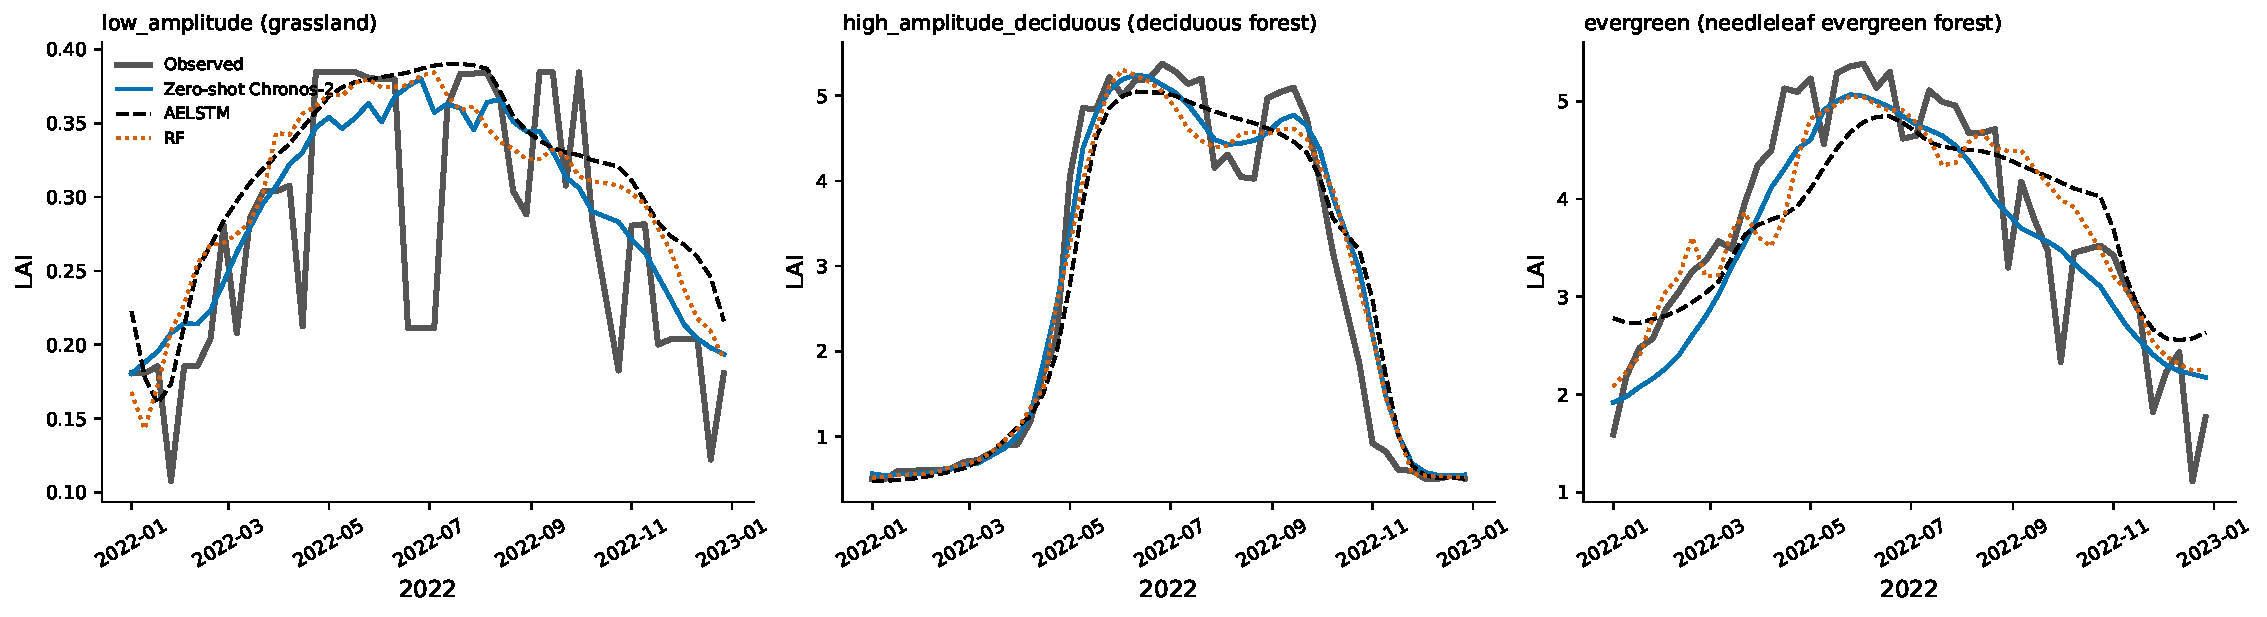
\includegraphics[width=\linewidth]{figures/prediction_examples.pdf}
  \caption{Representative LAI forecasting examples: observed vs.\ zero-shot Chronos-2 vs.\ AELSTM
  vs.\ the strongest supervised baseline, one panel per core pixel (\texttt{low\_amplitude},
  \texttt{high\_amplitude\_deciduous}, \texttt{evergreen}), 2022 held-out year.}
  \label{fig:prediction_examples}
\end{figure}

\Result{Zero-shot Chronos-2 ranks 1st on 2 of 3 pixels and is separated from the best method by
$0.00003$ $R^2$ on the third.}
\Interpretation{A pretrained, general-purpose time-series representation transfers to LAI
forecasting without any task-specific training.}
\Hypothesis{Broad pretraining on diverse time series may encode generic seasonal/periodic
structure that is also present, and exploitable, in vegetation phenology -- this has not been
demonstrated directly here and remains a hypothesis, not a result.}

\subsection{Comparison with supervised baselines}
\label{sec:results-comparison}

\Cref{tab:main_comparison} gives the full per-pixel ranking. Across the 3 shared pixels,
zero-shot Chronos-2 has the lowest (best) and most consistent mean rank of any method (1.33, std
0.58); the published AELSTM architecture itself never places better than 8th of 10 at any pixel.

\begin{figure}[t]
  \centering
  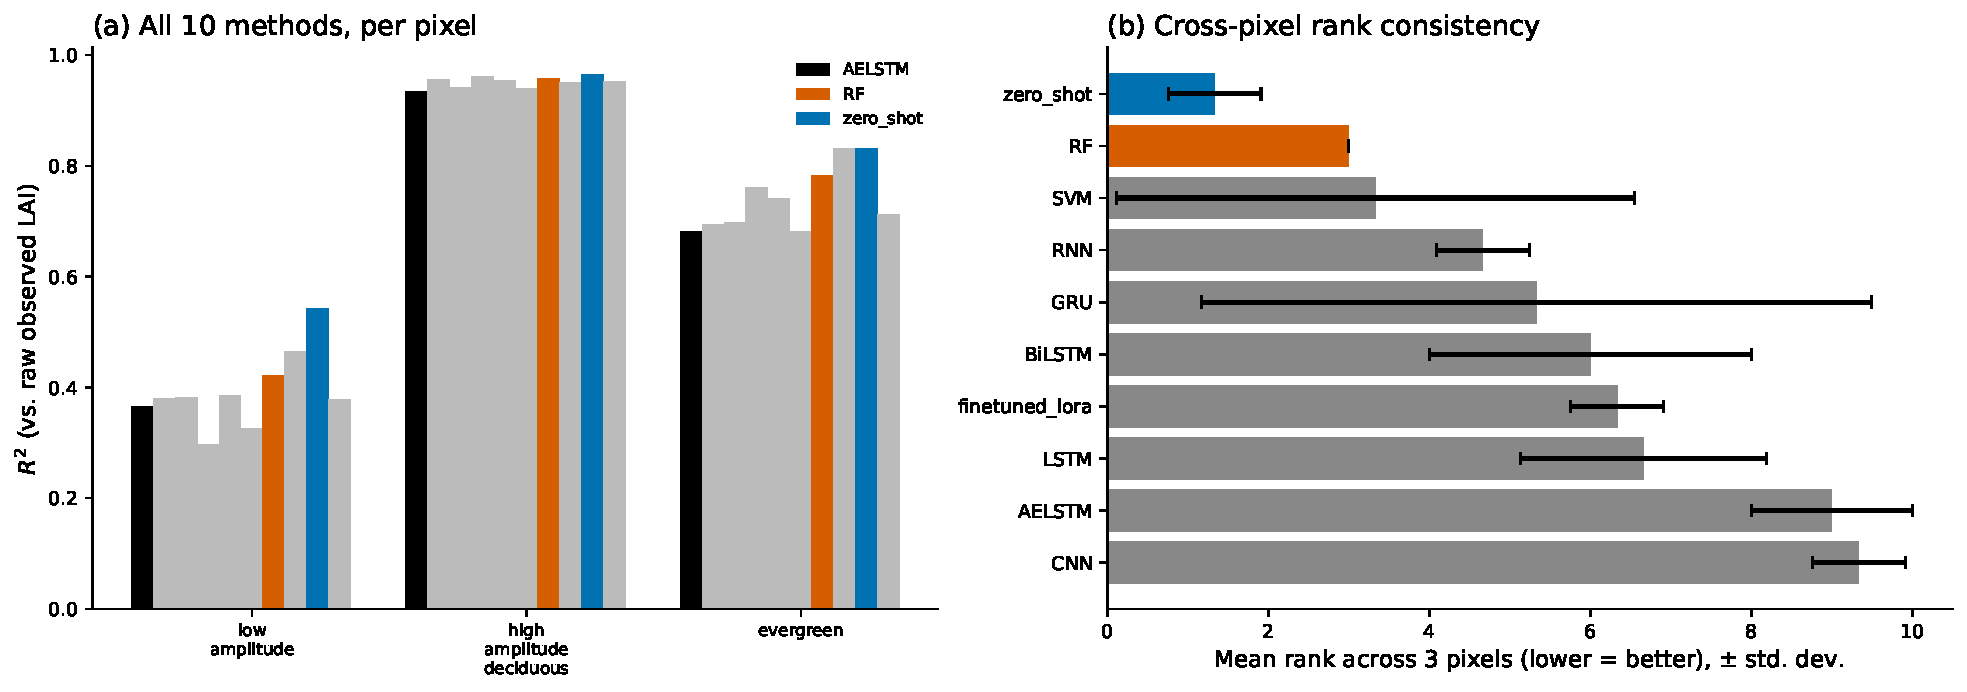
\includegraphics[width=\linewidth]{figures/baseline_comparison.pdf}
  \caption{Zero-shot Chronos-2 vs.\ 8 supervised baselines, rank consistency across the 3 core
  pixels, rebuilt from the authoritative raw-observation comparison
  (\texttt{outputs/fair\_comparison\_vs\_raw\_observations.csv}) -- \emph{not} the naive,
  smoothed-target comparison the baseline project's own pipeline reports internally.}
  \label{fig:baseline_comparison}
\end{figure}

\textbf{This advantage is not evidence of purely architectural superiority.} Chronos-2 is given
the actual future climate as a known covariate; none of the eight baselines have a mechanism to
use this information at all, by design -- they forecast from past climate only. The single
largest identifiable contributor to Chronos-2's advantage is this task asymmetry, not an implicit
claim that Chronos-2 ``predicts LAI better from the same information,'' because it does not
receive the same information. What remains genuinely notable, and defensible independent of the
covariate asymmetry, is that a \textbf{zero-shot, untrained} model is competitive at all against
eight specialized models each trained from scratch on the target pixel.

\Result{Zero-shot Chronos-2 is the best or tied-best model on 3/3 tested pixels, with future
climate as an input the baselines lack.}
\Interpretation{When reliable future meteorological forcing is available (seasonal forecasts,
scenario analysis), a foundation model with native covariate support is a strong practical choice
-- a claim about deployment usefulness under a specific information regime, not a head-to-head
architecture verdict.}

% Table 2: Zero-shot Chronos-2 vs. 8 supervised baselines, single 2022 held-out year
% Source (verified against CSV during audit): outputs/fair_comparison_vs_raw_observations.csv
\begin{table*}[t]
\centering
\caption{Zero-shot Chronos-2 vs.\ eight supervised baselines, single 2022 held-out year, all
methods scored against raw (unsmoothed) observed LAI. Baselines are trained from scratch per
pixel on past climate only; Chronos-2 additionally receives the actual future climate as a known
covariate (see \S\ref{sec:results-comparison} for the resulting interpretive caveat). Only the
top-2 and bottom-2-ranked methods per pixel are shown for space; the full 10-method table is
provided in the project repository. Bold: best result per pixel.}
\label{tab:main_comparison}
\begin{tabular}{@{}llrrrrrr@{}}
\toprule
Pixel & Model & RMSE & MAE & MAPE (\%) & R$^2$ & Pearson $r$ & Rank (of 10) \\
\midrule
\multirow{4}{*}{\texttt{low\_amplitude}}
 & \textbf{Zero-shot Chronos-2} & \textbf{0.0580} & \textbf{0.0396} & 17.94 & \textbf{0.542} & 0.760 & \textbf{1} \\
 & SVM & 0.0627 & 0.0464 & 21.11 & 0.465 & 0.719 & 2 \\
 & LoRA fine-tuned Chronos-2 & 0.0675 & 0.0530 & 20.61 & 0.379 & 0.649 & 7 \\
 & AELSTM & 0.0683 & 0.0487 & 23.15 & 0.365 & 0.749 & 8 \\
\midrule
\multirow{4}{*}{\texttt{high\_amplitude\_deciduous}}
 & \textbf{Zero-shot Chronos-2} & \textbf{0.372} & \textbf{0.246} & 14.14 & \textbf{0.965} & 0.984 & \textbf{1} \\
 & GRU & 0.393 & 0.286 & 14.44 & 0.961 & 0.982 & 2 \\
 & LoRA fine-tuned Chronos-2 & 0.439 & 0.286 & 16.05 & 0.952 & 0.976 & 6 \\
 & AELSTM & 0.513 & 0.333 & 17.81 & 0.934 & 0.967 & 10 \\
\midrule
\multirow{4}{*}{\texttt{evergreen}}
 & SVM & \textbf{0.4849} & 0.361 & 12.14 & \textbf{0.832} & 0.915 & 1 \\
 & Zero-shot Chronos-2 & 0.4850 & 0.426 & 14.02 & 0.832 & 0.930 & 2 \\
 & LoRA fine-tuned Chronos-2 & 0.635 & 0.531 & 16.53 & 0.712 & 0.878 & 6 \\
 & AELSTM & 0.668 & 0.526 & 18.12 & 0.681 & 0.846 & 9 \\
\bottomrule
\end{tabular}

\vspace{0.5em}
\begin{tabular}{@{}lrr@{}}
\multicolumn{3}{l}{\textit{Mean rank across all 3 pixels (of 10 methods), most consistent methods only}} \\
\toprule
Model & Mean rank & Std.\ dev.\ \\
\midrule
\textbf{Zero-shot Chronos-2} & \textbf{1.33} & \textbf{0.58} \\
Random Forest & 3.00 & 0.00 \\
AELSTM (published architecture) & 9.00 & 1.00 \\
\bottomrule
\end{tabular}
\end{table*}


\subsection{Temporal and spatial robustness}
\label{sec:results-robustness}

Across all 330 LOYO-CV folds (\Cref{tab:loyo}), zero-shot Chronos-2 has the second-lowest mean
rank (3.70 of 10, behind only Random Forest's 3.39) but the single highest top-3 finish rate of
any method (21/33 = 64\%, vs.\ RF's 20/33 = 61\%) -- the two lowest-mean-rank methods in the
entire study. Two folds are severe, genuine outliers ($z < -2.8$ on a per-pixel-normalized
difficulty score): \texttt{evergreen}/2012 (a real, sustained 2011--2012 U.S.\ Southeast drought,
unlike anything in 2000--2011 training data) and \texttt{low\_amplitude}/2018 (not a climate
anomaly -- an erratic, low-signal LAI trajectory at an already-low-amplitude pixel). On the
drought fold, both Chronos-2 variants rank 9th and 10th (worst) of 10; on the noisy fold,
zero-shot ranks 1st. No single year is difficult at more than one pixel simultaneously.

\begin{figure}[t]
  \centering
  \begin{subfigure}[b]{0.48\linewidth}
    \centering
    
\includegraphics[width=\linewidth]{figures/loyo_r2_distributions.pdf}
    \caption{$R^2$ distributions, all 10 methods $\times$ 3 pixels, 11 folds each.}
    \label{fig:loyo_r2_distributions}
  \end{subfigure}
  \hfill
  \begin{subfigure}[b]{0.48\linewidth}
    \centering
    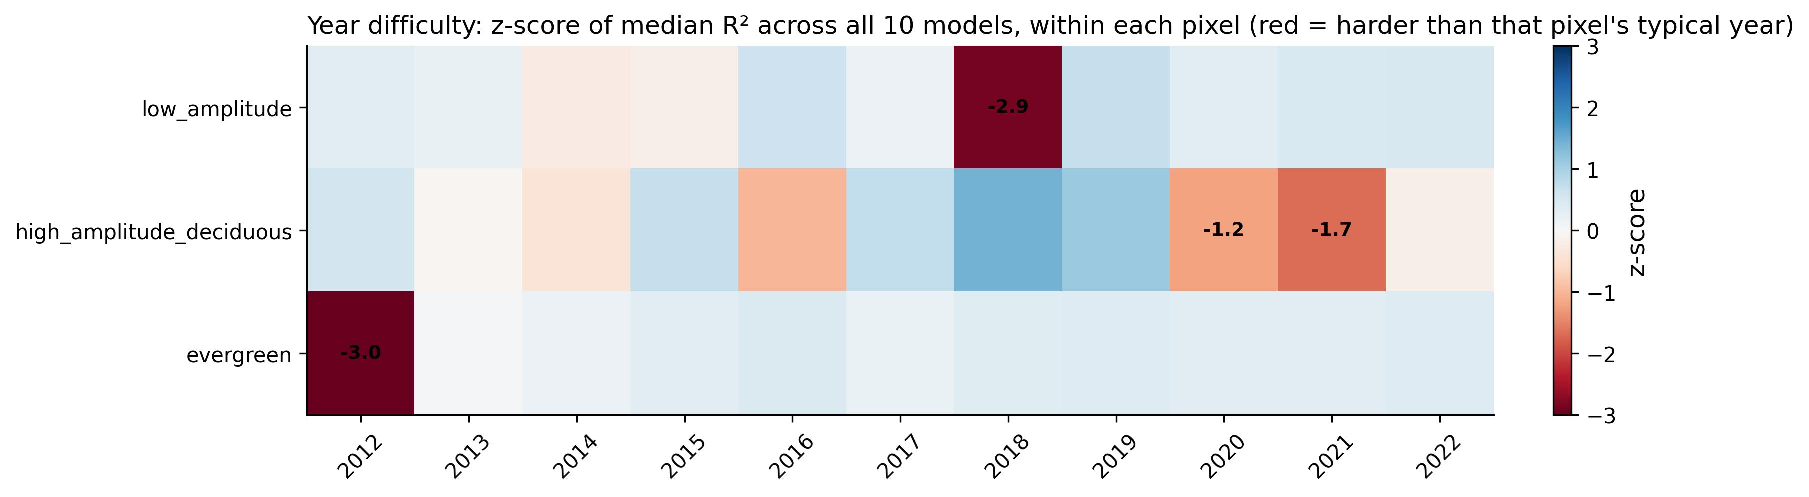
\includegraphics[width=\linewidth]{figures/loyo_year_difficulty.pdf}
    \caption{Per-pixel-normalized year-difficulty heatmap (z-score of median $R^2$).}
    \label{fig:loyo_year_difficulty}
  \end{subfigure}
  \caption{Chronos-2 performance across years (LOYO-CV, 2012--2022).}
  \label{fig:loyo_results}
\end{figure}

% Table 3: LOYO-CV performance summary (330 folds: 3 pixels x 11 years x 10 methods)
% Source (verified against CSV during audit): outputs/loyo_cv/comparison/loyo_summary_mean_std.csv,
%   LOYO_CV_FINDINGS.md Sec. 4
\begin{table*}[t]
\centering
\caption{Leave-one-year-out cross-validation (2012--2022, fixed 12-year rolling training window
immediately preceding each held-out year), 330 fold results (3 pixels $\times$ 11 years
$\times$ 10 methods). Panel (a): zero-shot Chronos-2's R$^2$ distribution per pixel across its 11
folds. Panel (b): cross-fold rank consistency across all 33 folds per method (top-2 and
bottom-2-ranked of 10 methods shown; full ranking in the project repository).}
\label{tab:loyo}
\begin{minipage}{\textwidth}
\centering
\textbf{(a) Zero-shot Chronos-2 R$^2$ distribution, per pixel, 11 folds each}\\[0.3em]
\begin{tabular}{@{}lrrrrr@{}}
\toprule
Pixel & Mean & Median & Std.\ dev.\ & Min & Max \\
\midrule
\texttt{low\_amplitude} & 0.317 & 0.387 & 0.388 & $-$0.717 & 0.645 \\
\texttt{high\_amplitude\_deciduous} & 0.957 & 0.961 & 0.023 & 0.896 & 0.985 \\
\texttt{evergreen} & $-$0.134 & 0.583 & 2.495 & $-$7.637 & 0.900 \\
\bottomrule
\end{tabular}

\vspace{1em}
\textbf{(b) Cross-fold rank consistency, all 33 folds (3 pixels $\times$ 11 years)}\\[0.3em]
\begin{tabular}{@{}lrrrr@{}}
\toprule
Model & Mean rank (of 10) & Std.\ rank & Top-3 finishes & Bottom-3 finishes \\
\midrule
Random Forest & 3.39 & 2.24 & 20/33 (61\%) & 3 \\
\textbf{Zero-shot Chronos-2} & \textbf{3.70} & 2.96 & \textbf{21/33 (64\%)} & 6 \\
LoRA fine-tuned Chronos-2 & 5.76 & \textbf{3.66 (highest)} & 13 & 15 \\
AELSTM (published architecture) & 7.00 & 2.33 & 2 & 12 \\
CNN & 7.48 & 2.37 & 2 & 19 \\
\bottomrule
\end{tabular}
\end{minipage}
\end{table*}


\Result{Chronos-2 is the two worst-of-ten methods on the one severe climate-anomaly fold in this
dataset, and the single best method on a different, non-anomalous but noisy fold.}
\Interpretation{Chronos-2 has no general ``robustness bonus'' to anomalous years; its overall edge
over the baseline family comes from typical years, not special resilience to distribution shift.}
\Hypothesis{Models with more explicit within-training exposure to anomaly-adjacent dynamics
(e.g.\ SVM, which degrades most gracefully on the drought fold) may encode features less reliant
on a ``normal seasonal cycle'' prior -- untested directly here.}

Spatially, a single LoRA adapter fit on \texttt{evergreen} and deployed \textbf{without
retraining} at \texttt{evergreen\_west} ($\sim$3{,}700\,km away, same vegetation type) achieves
$R^2 = 0.823$, fractionally exceeding a separately-fit target-local adapter ($R^2 = 0.819$) -- the
best spatial generalization of any of 9 methods compared, against AELSTM's own collapse to
negative $R^2$ under the identical test.

\begin{figure}[t]
  \centering
  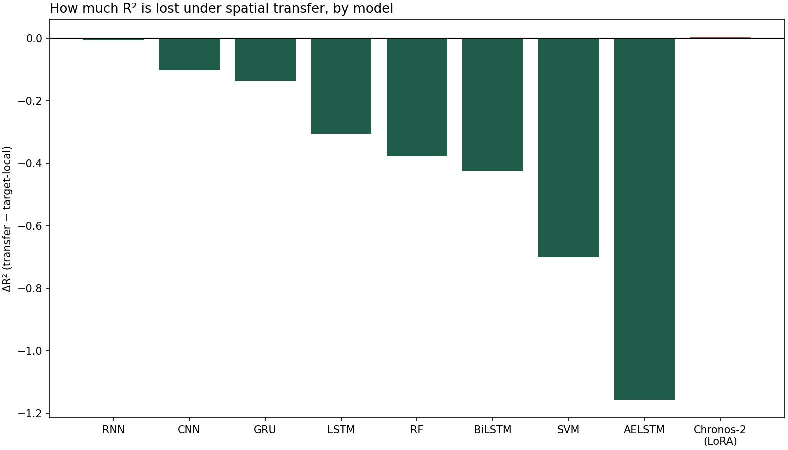
\includegraphics[width=0.7\linewidth]{figures/spatial_transfer.pdf}
  \caption{Spatial transfer: $\Delta R^2$ (transfer $-$ target-local), all 9 methods, same axis.
  Chronos-2 LoRA's transfer loss is statistically flat at zero; every AELSTM-family model loses
  more, and AELSTM itself collapses to negative $R^2$.}
  \label{fig:spatial_transfer}
\end{figure}

\subsection{Performance across vegetation and LAI regimes}
\label{sec:results-regimes}

Performance is strongly pixel-dependent: $R^2$ spans roughly 0.5 (\texttt{low\_amplitude}, a
sparse, low-signal grassland pixel) to 0.97 (\texttt{high\_amplitude\_deciduous}, a strong,
high-amplitude seasonal cycle) for essentially every method tested, including Chronos-2 -- a far
larger range than the spread between methods at any single pixel (\Cref{sec:results-adaptation}
confirms this holds under adaptation too). Predictor-sensitivity analysis (zero-shot Chronos-2
among 9 methods) finds $\mathit{srad}$ (downward shortwave radiation) the only predictor whose
removal consistently hurts at every pixel; temperature importance is almost entirely
pixel-specific (critical at \texttt{low\_amplitude}, unimportant-to-mildly-helpful-when-removed
elsewhere); and a leaner 5-predictor set (dropping $\mathit{vs}$, $\mathit{pr}$) improves mean
$R^2$ at all 3 pixels simultaneously, a validated actionable finding independent of which
forecasting model is used.

\begin{figure}[t]
  \centering
  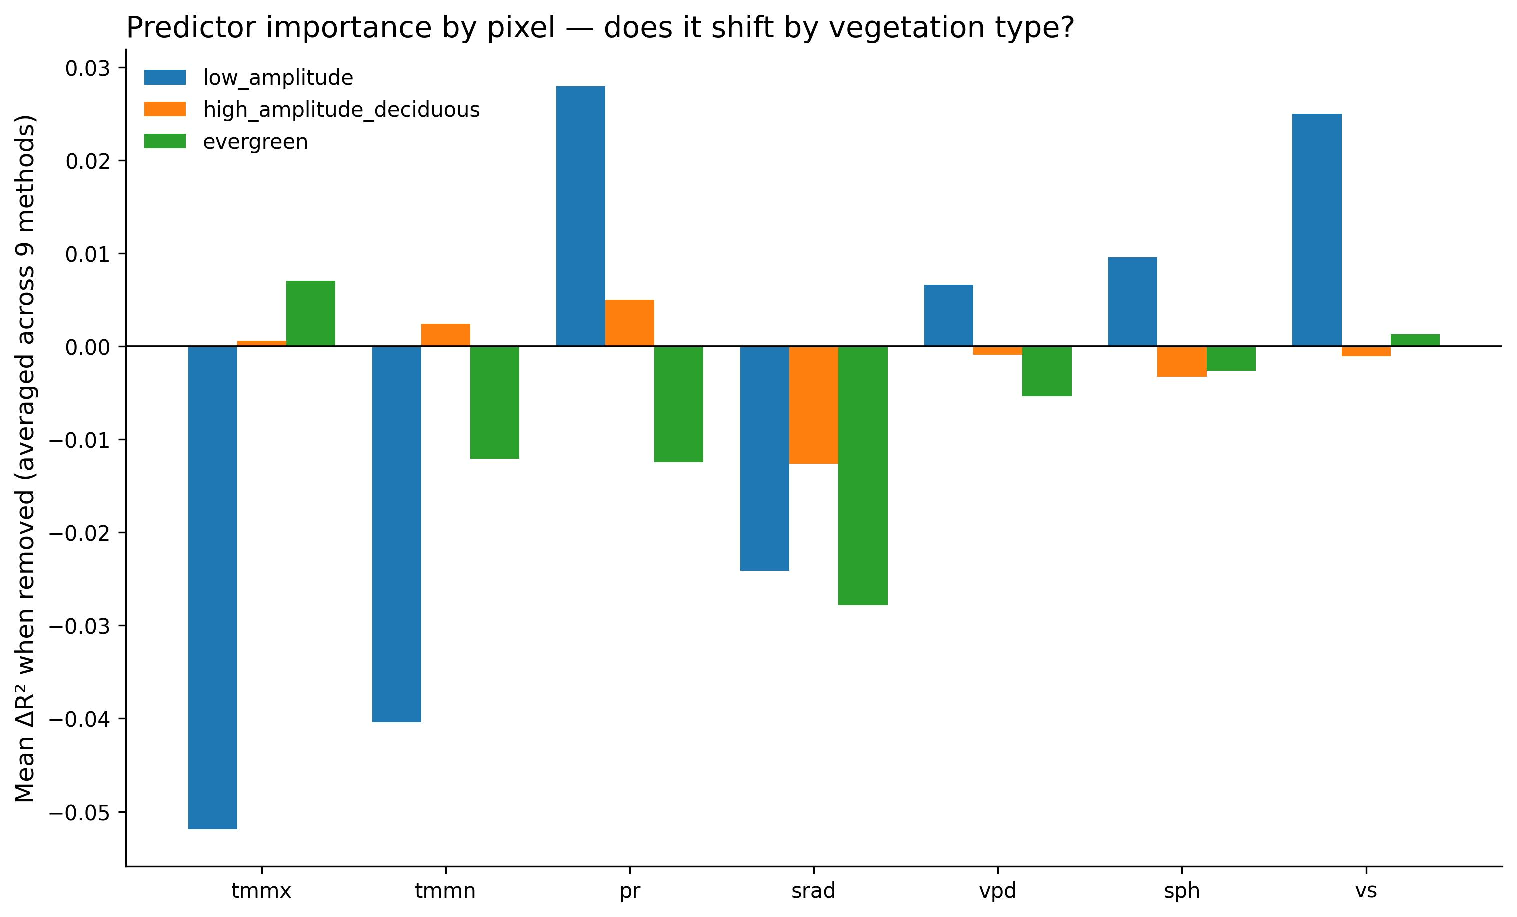
\includegraphics[width=\linewidth]{figures/predictor_importance.pdf}
  \caption{Mean $\Delta R^2$ when each of the 7 climate predictors is removed (leave-one-out),
  broken down by pixel. $\mathit{srad}$ is the only predictor with a consistently negative
  $\Delta R^2$ across all three vegetation regimes.}
  \label{fig:predictor_importance}
\end{figure}

\subsection{Can parameter adaptation improve Chronos-2?}
\label{sec:results-adaptation}

\textbf{No adaptation method tested in this project consistently beats zero-shot Chronos-2.}
\Cref{tab:adaptation} summarizes. Original (unvalidated) LoRA fine-tuning is uniformly worse
($\Delta R^2 = -0.163, -0.014, -0.120$ across the 3 pixels). Adding validation-based checkpoint
selection recovers most, but not all, of this gap on the two pixels where it was worst
(\texttt{low\_amplitude}: $-0.042$ remaining; \texttt{evergreen}: $-0.003$, effectively closed)
without ever crossing zero-shot outright. Extending to six further PEFT methods spanning a
1{,}500-fold range of trainable-parameter count (8{,}352 to 13{,}093{,}536) -- additive low-rank
(DoRA), multiplicative rescaling (IA3), bias-only (BitFit), normalization-only (LN-Tuning),
shared-random-projection (VeRA), and full-weight partial fine-tuning -- finds the same pattern:
mean $R^2$ across all fine-tuning variants is uniformly below zero-shot's 0.780, and only one
method/pixel combination (DoRA on \texttt{evergreen}, $+0.0026$) beats zero-shot at all, by a
margin plausibly attributable to noise. Trainable-parameter count is, at best, a weak and
inconsistent predictor of outcome (pooled $r = +0.10$ with test $R^2$; the sign of the correlation
even flips between pixels).

The vegetation-composition-conditioning experiments extend this finding with a mechanistic
explanation rather than merely replicating it. A single-pixel, constant PFT covariate is
\textbf{architecturally provably erased} by Chronos-2's per-series InstanceNorm
(\Cref{eq:in-loc}--\Cref{eq:in-scaled}) -- confirmed by direct source inspection and an exact,
8-decimal-place-zero empirical perturbation test. Fixing this with a FiLM-conditioning head
(\Cref{eq:film}) genuinely capable of learning a PFT-dependent response (verified via a smoke test
and a deliberately-overfit checkpoint that shows large, physically plausible sensitivity, up to
0.63 LAI units) still fails to produce a validated improvement: across four architecturally
distinct conditioning designs -- spanning an 8$\times$ range in trainable parameters, with and
without dropout and weight decay -- three of four overfit within the first training step even
given 8 rolling training windows (4$\times$ more temporal supervision than the initial 2-window
design). The fourth (\texttt{low\_rank}, a rank-8-bottleneck design) is the only architecture that
trains past step 0 -- and the paper's decisive result is that an identical \texttt{low\_rank} head
trained on \textbf{randomly shuffled} PFT-to-pixel assignments improves 2022 $R^2$ by $+0.0024$,
marginally \emph{more} than the real-PFT condition's $+0.0022$, with no statistically detectable
difference between them (paired $t$-test $p=0.245$, Wilcoxon $p=0.663$, $n=70$ pixels; 31/70
pixels favor real PFT, 39/70 favor shuffled). Neither seasonal-phase breakdown nor
mixed-vs-pure-pixel entropy analysis reveals any shuffle-surviving signal.

\begin{figure}[t]
  \centering
  \begin{subfigure}[b]{0.48\linewidth}
    \centering
    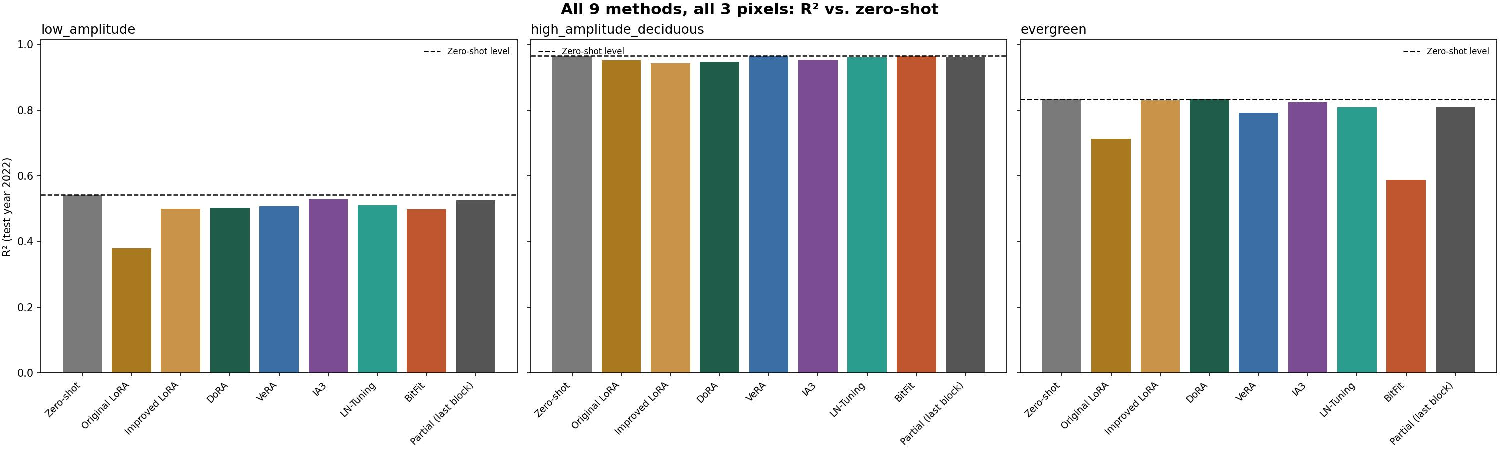
\includegraphics[width=\linewidth]{figures/adaptation_results.pdf}
    \caption{$R^2$, all 9 fine-tuning/PEFT methods $\times$ 3 pixels, vs.\ the zero-shot line.}
    \label{fig:adaptation_peft}
  \end{subfigure}
  \hfill
  \begin{subfigure}[b]{0.48\linewidth}
    \centering
    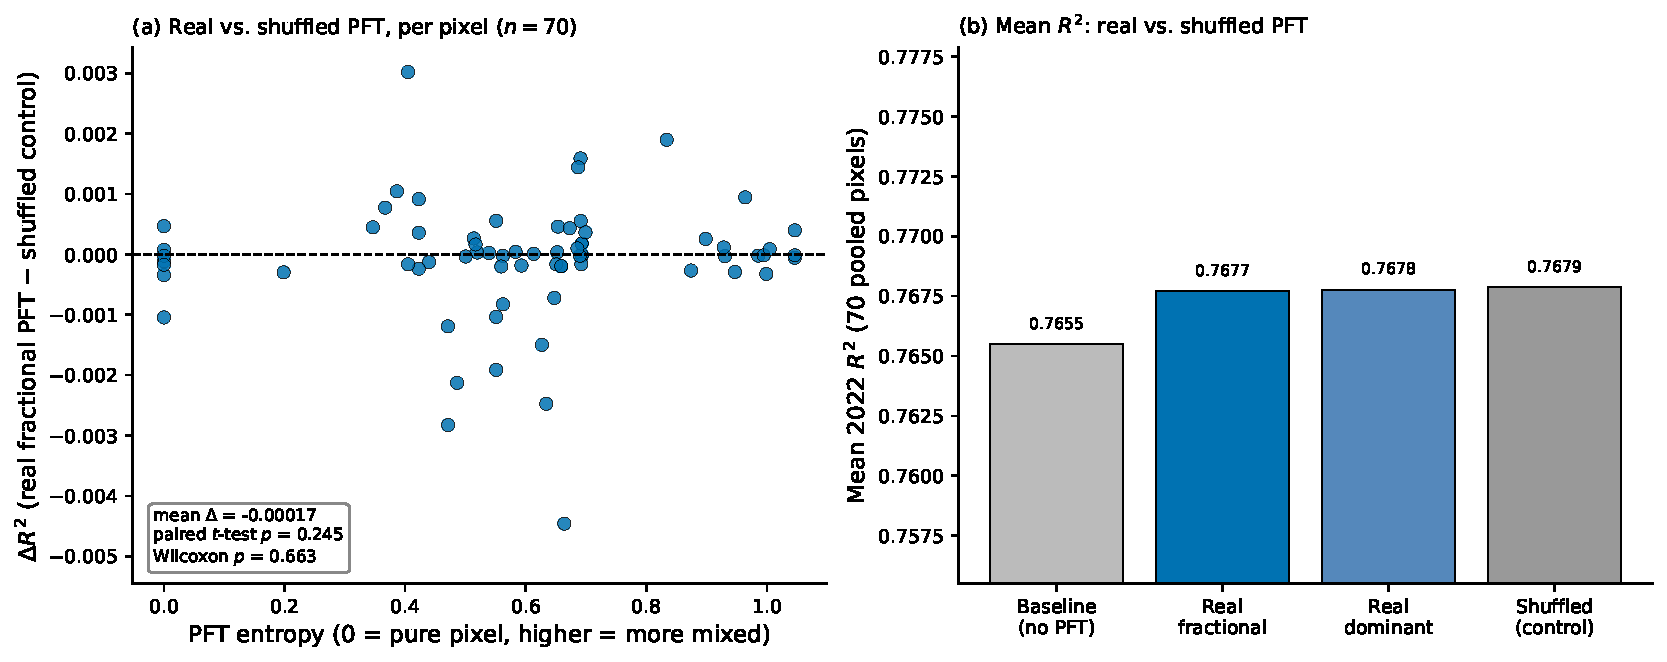
\includegraphics[width=\linewidth]{figures/pft_shuffle_control.pdf}
    \caption{Real vs.\ shuffled PFT, per-pixel $\Delta R^2$ vs.\ baseline, $n=70$.}
    \label{fig:pft_shuffle_control}
  \end{subfigure}
  \caption{Zero-shot vs.\ adaptation: (a) the 7-method PEFT sweep; (b) the decisive PFT-conditioning
  shuffled-assignment control.}
  \label{fig:adaptation_combined}
\end{figure}

\Result{Seven distinct parameter-efficient fine-tuning methods and four
vegetation-composition-conditioning architectures were tested under a validated, test-isolated
protocol; none consistently beats zero-shot Chronos-2, and a randomized shuffled-assignment
control shows the one architecture that does train past initialization derives no detectable
benefit from real vegetation-composition information over scientifically meaningless input.}
\Interpretation{This is not evidence that any single adaptation method or covariate design was
chosen poorly -- the shuffle control specifically rules out ``wrong information, right mechanism''
as the explanation. Task-specific adaptation did not consistently improve upon the zero-shot
model, highlighting the strength of the pretrained representation and the difficulty of improving
a strong foundation-model baseline with limited target-domain data.}
\Hypothesis{Pretrained zero-shot Chronos-2 may already sit close to this dataset's achievable
ceiling; any small amount of gradient-trained conditioning capacity added on top, on data this
limited, may nudge predictions by a similarly-sized, generic amount regardless of what
information drives it -- a hypothesis directly motivated by, but not fully proven beyond, the
shuffle-control result and the PEFT sweep's parameter-count-independence finding taken together.}

% Table 4: Zero-shot vs. every parameter-adaptation method tested
% Source (verified against CSV during audit): outputs/advanced_finetuning/final_ranking_table.csv,
%   outputs/pft_v2/final_2022_summary.csv, outputs/pft_v2/real_vs_shuffled_ttest.csv
\begin{table*}[t]
\centering
\caption{Zero-shot vs.\ every parameter-adaptation method tested, mean across the 3 core pixels,
single 2022 held-out year, validated protocol (chronological pre-2022 validation split, early
stopping, test set isolated from all selection decisions) for every method except the original
(unvalidated) LoRA row. Panel (a) sorted by mean R$^2$. Panel (b): the decisive PFT-conditioning
randomized control, 70 pooled pixels, \texttt{low\_rank} architecture (the only one of four tested
that trained past initialization; see \S\ref{sec:results-adaptation}).}
\label{tab:adaptation}
\textbf{(a) Standard and advanced parameter-efficient fine-tuning (PEFT)}\\[0.3em]
\begin{tabular}{@{}lrrrl@{}}
\toprule
Method & Trainable params.\ & Mean R$^2$ & $\Delta$ vs.\ zero-shot & Pixels beating zero-shot \\
\midrule
\textbf{Zero-shot} & --- & \textbf{0.780} & --- & --- \\
IA3 & 73{,}728 & 0.769 & $-$0.011 & 0/3 \\
Partial (last block) & 13{,}093{,}536 & 0.766 & $-$0.014 & 0/3 \\
DoRA & 1{,}280{,}976 & 0.761 & $-$0.019 & 1/3 \\
LN-Tuning & 28{,}416 & 0.760 & $-$0.020 & 0/3 \\
Improved LoRA (validated) & --- & 0.757 & $-$0.023 & 0/3 \\
VeRA & 98{,}896 & 0.755 & $-$0.025 & 0/3 \\
BitFit & 8{,}352 & 0.683 & $-$0.097 & 0/3 \\
Original LoRA (unvalidated) & 1{,}280{,}976 & 0.681 & $-$0.099 & 0/3 \\
\bottomrule
\end{tabular}

\vspace{1.2em}
\textbf{(b) PFT-composition conditioning: real vs.\ shuffled-assignment control}\\[0.3em]
\begin{tabular}{@{}lrrl@{}}
\toprule
Condition & Mean 2022 R$^2$ & $\Delta$ vs.\ baseline & Statistical test (real vs.\ shuffled) \\
\midrule
Baseline (zero-shot, no PFT) & 0.7655 & --- & --- \\
+ Real fractional PFT & 0.7677 & +0.0022 & --- \\
+ Real dominant PFT & 0.7678 & +0.0023 & --- \\
+ \textbf{Shuffled PFT (control)} & \textbf{0.7679} & \textbf{+0.0024} & paired $t$-test $p=0.245$, Wilcoxon $p=0.663$ ($n=70$) \\
\bottomrule
\end{tabular}
\end{table*}


\subsection{Failure cases and challenging environmental conditions}
\label{sec:results-failure}

The \texttt{evergreen}/2012 LOYO-CV failure (zero-shot $R^2 = -7.64$; original LoRA
$R^2 = -8.29$, the single worst score of all 9 methods compared this way) is mechanistically
resolved by the leakage diagnostic: allowing 2012 to participate in LoRA fitting (a deliberate
leakage condition, \textbf{not} a valid evaluation) recovers RMSE by 59.9\% and $R^2$ to $-0.50$
-- the second-largest recovery of 9 methods tested this way (behind only Random Forest, $+8.01$),
landing squarely in the middle of the baseline pack rather than uniquely bad. Both the recovering
and the original failure are large and consistent across essentially every architecture tested
(tree ensemble, six neural sequence models, and a large pretrained transformer), which is the
signature of a shared external cause -- the 2012 drought being genuinely unlike anything in
2000--2011 training data -- rather than an architecture-specific representational limitation.

\begin{figure}[t]
  \centering
  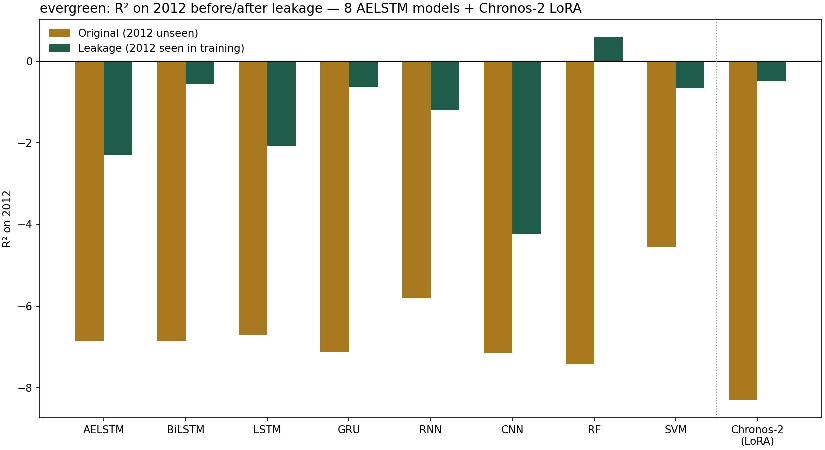
\includegraphics[width=0.7\linewidth]{figures/leakage_diagnostic.pdf}
  \caption{Leakage diagnostic, \texttt{evergreen}/2012: cross-project $R^2$ comparison, Chronos-2
  LoRA alongside all 8 AELSTM-family models, ``2012 unseen'' vs.\ ``2012 seen in training''
  (deliberate leakage; not a valid evaluation protocol -- diagnostic only).}
  \label{fig:leakage_diagnostic}
\end{figure}

% =============================================================================
\section{Discussion}
\label{sec:discussion}
% =============================================================================

\textbf{Why might Chronos-2 transfer successfully to LAI?} Vegetation phenology is strongly
seasonal and climate-driven, structurally similar to many series in a broad pretraining corpus;
Chronos-2's native handling of known future covariates directly matches this paper's forecasting
formulation. The strong zero-shot baseline (\Cref{sec:results-zeroshot,sec:results-comparison})
suggests pretrained time-series representations can transfer effectively to this domain without
modification -- a result consistent with, and extending to a new domain, prior evidence that
Chronos-2 zero-shot performance is strong relative to fine-tuning on small datasets
\citep{arxiv2607.23146}.

\textbf{What does strong zero-shot performance imply, and what doesn't it imply?} It implies that,
for practitioners with access to reliable future meteorological forcing, a general-purpose TSFM
is a credible default without investing in a purpose-built architecture or a target-domain
training pipeline. It does not imply Chronos-2's architecture is intrinsically superior at
sequence modeling in general -- this project's comparison is not same-task
(\Cref{sec:results-comparison}), and the baselines' collapse under spatial transfer (in sharp
contrast to Chronos-2's success, \Cref{sec:results-robustness}) suggests at least some of them
were fitting genuinely useful, if non-transferable, location-specific structure that a
covariate-blind pure zero-shot comparison cannot credit them for.

\textbf{When do supervised models retain advantages?} Random Forest is the single most consistent
performer across the entire LOYO-CV study (lowest rank volatility, comparable mean rank to
Chronos-2) and degrades most gracefully of all 10 methods on the one severe drought fold --
evidence that a simple, well-regularized supervised model trained directly on the target series
retains real advantages in anomalous conditions a pretrained zero-shot model has not encountered.

\textbf{Why might fine-tuning fail to improve a strong pretrained model, here specifically?} Three
lines of evidence converge: (1) each fine-tuning run adapts on a single, short ($\sim$1{,}000-point)
series -- the scenario Chronos-2's own documentation identifies as a regime where fine-tuning
``may not improve over zero-shot (and may even worsen accuracy sometimes)''; (2)
trainable-parameter count is a weak, inconsistent predictor of outcome across a 1{,}500$\times$
range, arguing against ``insufficient capacity'' as the explanation; (3) the PFT shuffle control
directly demonstrates that added conditioning capacity produces a similar effect size whether or
not it carries real information, which is difficult to reconcile with any story in which the
\emph{specific} information being added is the limiting factor. Together, these support the
hypothesis that the binding constraint is the \textbf{combination} of a strong pretrained prior
and a small amount of target-domain data, not any one adaptation method's design.

\textbf{What environmental regimes remain difficult?} Sustained, multi-month anomalies genuinely
absent from a model's training window (\Cref{sec:results-failure}) remain hard for every method
tested, Chronos-2 included, and Chronos-2 shows no special resistance to this specific failure
mode -- an important tempering of the paper's otherwise favorable robustness story
(\Cref{sec:results-robustness}).

\textbf{Implications for future vegetation foundation-model research.} The clearest actionable
implication is methodological: any future claim that an adaptation or conditioning method improves
a strong pretrained forecaster on limited data should be checked against a randomized-assignment
control before being reported as a positive result -- this project's own preliminary multi-pixel
PFT-conditioning experiment would have been reported as a promising, if inconclusive, positive
direction without the shuffle control added afterward, and that control reversed the reading
entirely.

% =============================================================================
\section{Limitations}
\label{sec:limitations}
% =============================================================================

\begin{itemize}
  \item \textbf{Small core sample.} The primary cross-model comparison rests on 3 pixels; rank
    volatility among several baselines (e.g., GRU swinging from rank 2 to rank 10) is a direct
    warning that single-digit-pixel-count rankings, including ``Chronos-2 is best,'' could shift
    with more locations. Three additional pre-selected pixels exist but have not been run through
    Chronos-2.
  \item \textbf{Task asymmetry.} Chronos-2's headline comparison against the baselines is not
    same-information; the baselines never receive future climate. This is repeatedly flagged
    in-text (\Cref{sec:results-comparison}) and should not be read as a pure architecture verdict.
  \item \textbf{Geographic scope.} All experiments are CONUS-only (HiQ-LAI/gridMET coverage); a
    global ERA5-based generalization study is underway but has produced no results as of this
    writing.
  \item \textbf{Single pretrained checkpoint, unseeded fine-tuning stochasticity.} All results use
    one Chronos-2 checkpoint (\texttt{amazon/chronos-2}); the fine-tuning dataset's
    training-window sampling is not seeded across runs, introducing run-to-run noise on the order
    of the leakage diagnostic's $\sim$0.6 $\Delta R^2$ reproduction gap between two nominally
    identical fine-tuning conditions.
  \item \textbf{PFT screening is not exhaustive.} Four conditioning architectures and two
    learning rates each were tested; conditioning additional (covariate) rows beyond the target
    row, and cross-attention/mixture-of-experts-style gating, were reasoned about but not run.
\end{itemize}

% =============================================================================
\section{Conclusion}
\label{sec:conclusion}
% =============================================================================

Across a systematic evaluation spanning a single-year comparison, 330 leave-one-year-out
cross-validation folds, a long-distance spatial transfer test, and the most extensive adaptation
study conducted in this project -- seven parameter-efficient fine-tuning methods and four
vegetation-composition-conditioning architectures, including a randomized control -- zero-shot
Chronos-2 emerges as a strong, robust, and (with one important, honestly-reported exception:
sustained climate anomalies genuinely absent from its context) dependable LAI forecaster, on par
with the best supervised alternatives tested, without any task-specific training. Its zero-shot
representation appears to already be close to what limited-data adaptation on this dataset can
reach: not one of eleven distinct adaptation mechanisms tested consistently improves on it, and
the project's decisive randomized control shows that even a genuinely working conditioning
architecture derives no detectable benefit from real information over scientifically meaningless
input. For vegetation LAI forecasting specifically, and plausibly for other data-limited
Earth-system tasks with structurally similar covariates, these results support deploying
general-purpose, pretrained time-series foundation models zero-shot as a strong default,
reserving further adaptation effort for settings with substantially larger or more diverse
target-domain data than were available here.

% =============================================================================
\bibliographystyle{plainnat}
\bibliography{references}

\end{document}
